The multi-agent path finding problem (MAPF) is more challenging than the single-agent problem due to the high dimension of its configuration space. Broadly speaking, there are two approaches to solve this problem: planning and reacting. In the planning approach, collision-free paths are generated ahead of time, whereas the reactive approach uses online collision avoidance schemes while encountering hazardous situations. In this chapter, we introduce the various approaches of tackling problem. 

\section{Graph Search Methods}
These approaches compute the path by applying the graph-search algorithms on the configuration space of the multi-robot system, which is the Cartesian product of the configuration spaces of each robot. Here, robot-robot collisions are expressed as configuration space obstacles. The full configuration space grows exponentially with the number of robots, thus making the standard search algorithms computationally infeasible. 

It is not necessary to plan in this space as the robots are usually well separated in the workspace, and collisions are infrequent. Some works generate feasible results by exploiting this decoupled property of the system. In this section, we discuss two such methods: M* \cite{wagner2011m} and conflict based search \cite{sharon2015conflict}. These methods have proven to produce remarkable results for cases with high congestion. 
\subsection{M* Search}
Initially, M* algorithm plans for each robot separately, without considering collisions. This is a good starting point for multi-robot planning as no path can be cheaper than this. When collisions occur, planning is performed in the joint configuration space (see Figure.~\ref{fig:mstar}) of the robots involved in the collision while uninvolved robots proceed independently. When the collision is bypassed, planning continues to proceed in low dimensional individual spaces. 

\begin{figure}
    \centering
    \begin{subfigure}[b]{0.4\textwidth}
        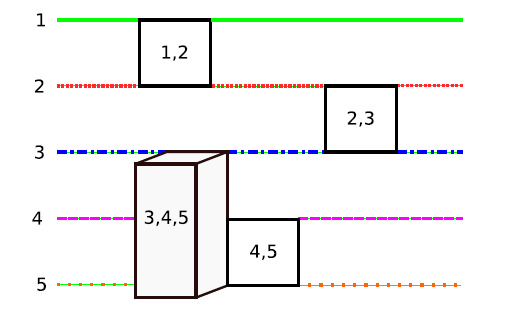
\includegraphics[width=\textwidth]{./images/m_star_a.png}
        \caption{Representation of search space in M* algorithm}
        \label{fig:mstara}
    \end{subfigure}
    ~ %add desired spacing between images, e. g. ~, \quad, \qquad, \hfill etc. 
    \begin{subfigure}[b]{0.55\textwidth}
        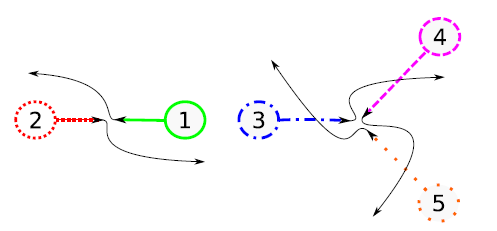
\includegraphics[width=\textwidth]{./images/m_star_b.png}
        \caption{Motion of multiple robots in the shared workspace}
        \label{fig:mstarb}
    \end{subfigure}
    \caption[Visualization of the variable dimensionality workspace in M* algorithm.]{Visualization of the variable dimensionality workspace in M* algorithm. When two robots collide, the local dimensionality is increased to 2 (represented by a square). Similarly, when three robots collide the dimensionality is 3 (cube). \cite{wagner2011m} }\label{fig:mstar}
\end{figure}

Like A* algorithm, M* explores a list of vertices sorted based on the sum of the cost of the cheapest path and a heuristic cost. M* considers only a limited set of neighbours determined by a \textit{collision set}, thus minimizing the dimensionality. M* can be seen as performing A* search in a  dynamically updating graph, $G^\#$. M* algorithm can handle problems involving a high number of robots, while retaining bounded optimality and \textit{completeness}. 


%M* algorithm was proven to be \textit{complete}. Moreover, it is capable of scaling to problems involving high dimension of robots, while maintaining completeness and bounded optimality. 
The uncertainties of the poses, inherent to robotics, was taken into consideration in UM* \cite{Wagner2017PathPF}. In this approach, planning is done in the belief space to account for the uncertainties. Then, a scheme similar to M* is implemented. 
\subsection{Conflict Based Search}
Conflict-Based Search (CBS) is a bounded sub-optimal two-level MAPF solver. The top level solves a binary \textit{constraint tree} (CT), whose nodes consists of a set of constraints, a single solution, and the cost of solution. The low level of CBS searches for a plan that satisfies all the constraints in a node $N$. If a node is conflict-free, it is returned as the solution. Otherwise, CBS splits node $N$ based on one of the conflicts. Let $<a_i, a_j, v, t>$ represent the conflict between agents $a_i$ and $a_j$ at vertex $v$ at time-step $t$. Now, $N$ is split into two children node, one with the constraint $<a_i, v, t>$ and the other with $<a_j,v,t>$. By doing so, the solver imposes a constraint on only one agent at a time. 

An example of this node expansion scheme is shown in Figure.~\ref{fig:cbs}. In this problem, each mouse (agent) must find a path to cheese (goal). Node $R$ is initialized with no constraints. The shortest paths generated has a collision $<1,2,D,2>$. Therefore, two nodes, $U$ and $V$, are generated with constraints $<1,D,2>$ and $<2,D,2>$ respectively. This leads to collision free solutions. As this search method is exponential in the number of conflicts encountered, as opposed to the number of agents, it leads to superior results. 

Since solving MAPF problems are optimally NP-hard, optimal solutions like M* and CBS are feasible only for low number of agents. Therefore, it is common to use bounded-suboptimal solutions for higher number of agents. Koenig et al. \cite{cohen2016bounded} uses user-provided highways to generate suboptimal paths for a large number of robots. 

The graph plans from these grid based search methods cannot be directly interpreted as trajectory results as they do not consider the kinematic and dynamics constraints of the robot. \cite{honig2016multi} deals with this problem by post-processing the output of the MAPF solvers using a simple temporal network. 

\begin{figure}
\centering
\includegraphics[width=0.6\textwidth]{./images/CBS}
\caption[Visualization of Conflict Based Search]{Visualization of Conflict Based Search (CBS): (I) MAPF instance, and (II) its Constraint-Tree (CT)}
\label{fig:cbs}
\end{figure}

\section{Continuous optimization schemes}
Some researchers the MAPF problem in a continuous setting by formulating it as an optimisation problem with the trajectories defined by its decision variables. These methods generate smooth solutions for small fleets of robots. 

D’Andrea et al. \cite{augugliaro2012generation}, solves this problem using sequential quadratic programming. Suppose we have $N$ vehicles, and $K$ time steps. The position of the vehicle $i$ at time-step $k$ is denoted as $p_i[k]$. The velocity and acceleration equations are:
\begin{align}
\begin{split}
&v_i[k+1]=v_i[k]+ha_i[k]\\
&p_i[k+1]=p_i[k] + hv_i[k] + \frac{h^2}{2}a_i[k],
\end{split}
\end{align}
The optimization variable $\chi\in \mathbb{R}^{3NK}$ is made of the accelerations of the vehicles at each time step. The velocity and acceleration of the vehicle $i$ at time $k$ can also be written as:
\begin{align}
\begin{split}
&v_i[k]=v[1] + h(a_i[1] + a_i[2] +\ldots+a_i[k-1])\\
&p_i[k]=p_i[1] + h(k-1)v_i[1] + \frac{h^2}{2}\left((2k-3)a_i[1] + (2k-5)a_i[2]+\ldots+a_i[k-1]\right))
\end{split}
\end{align}
The objective function is the sum of the total thrust at each step can be written as:
\begin{align}
f_0=\sum_{i=1}^N\sum_{k=1}^K\left\Vert a_i[k]+g\right\Vert
\end{align}
where, $g$ is the gravity vector. This function can be expressed as a quadratic function of the optimization variable $\chi$. The fixed initial and final states gives rise to some equality constraints. Similarly, the limits on the workspace, as well as the dynamics limits of the quadrotor creates inequality constraints on the position, velocity, acceleration, and jerk. If the robots should be at a safe distance of $R$ between each other to avoid collisions, the following non-convex constraint must be imposed:
\begin{align}
\Vert p_i[k]-p_j[k]\Vert_2 \geq R
\end{align} 
Using sequential convex programming, these constraints can be replaced with convex approximations around a previous solution $\chi^q$ using a first order Taylor expansion. The minimization problem can now be written as:
\begin{align}
\begin{split}
\min \quad &f_0(\chi) = \chi^\top P\chi + q^\top \chi + r \\
\text{s.t.} \quad &A_{eq}\chi=b_{eq}\\&A_{in}\chi\leq b_{in}
\end{split}
\end{align}
The optimum solution was found using QP. A demonstration of this method can be seen in Figure.~\ref{fig:sqp}.

\begin{figure}
\centering
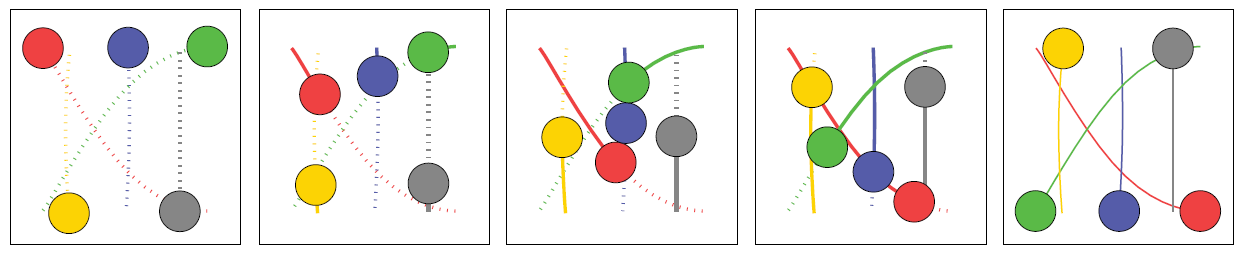
\includegraphics[width=\textwidth]{./images/dandrea_scp.png}
\caption[Multi-agent trajectory planning using sequential quadratic programming.]{Multi-agent trajectory planning using sequential quadratic programming. \cite{augugliaro2012generation}}
\label{fig:sqp}
\end{figure}

In \cite{mellinger2012mixed}, a Mixed-Integer Quadratic Program (MIQP) is solved to generate feasible paths. These methods are capable of creating smooth, optimal solutions. However, these methods are often tightly and hence do not scale  up well to large teams. 

\section{Planning with Goal Assignment}
In many applications of multi-agent systems, the agents are interchangeable. For instance, in case of first-response and search and rescue applications, the aim is to explore the maximum area with a limited number of robots. In the context of the path planning problem, this translates to having no one-to-one correlation between the initial and goal locations. Therefore, goal-assignment should also be a part of the planning algorithm to obtain the best results. 

Paradoxically, coupling the goal-assignment with trajectory planning reduces the complexity of the problem \cite{turpin2013trajectory}. Koenig et al. \cite{ma2016optimal} presented a Conflict-Based Min-Cost-Flow (CBM) algorithm to solve this problem. CBM works in two stages: in stage 1, min-cost max-flow algorithm \cite{goldberg1987solving} to assign the agents to goals, and in stage 2, CBS is used to find collision-free paths. This algorithm was proved to be complete and optimal, and demonstrated to be scalable. 

In \cite{turpin2014goal}, a graph $G$, which has the dimensionality of a single robot is first generated, and then the assignment problem is solved using Hungarian-algorithm \cite{kuhn1955hungarian}. Collisions are avoided by adding time offsets in the trajectories. This method was proven to have a computational complexity that is cubic in the number of robots, which is a significant improvement from the expected exponential complexity. However, due to the time offsets, this method leads to high execution time.
\section{Velocity Profile Methods}
Some researchers address this problem using velocity profile methods\cite{peng2005coordinating}. First, the optimal path for each robot is computed without considering robot-robot collisions. Then the robots are coordinated so that they do not collide. It must be noted that the robots always stay at their best paths. 

Let $\mathcal{S}_i=[0,1]$  be the set of parameters that represent the position of the robot along its trajectory. These parameters constitute the coordination space, with $s_{init}=(0,0,\ldots,0)$ and $s_{goal}=(1,1,\ldots,1)$. A collision pair $\mathcal{CP}_{ij}$ is defined as a pair of configurations where robots $\mathcal{A}_i$ and $\mathcal{A}_j$ collide. Each robots paths are decomposed into collision segments and collision-free segments. 

Since each robot has dynamics constraints on its velocity and accelerations, there is an upper and lower limit to the time in which it can traverse a segment $k$ represented by $\Delta T_{ik}^{max}$ and $\Delta T_{ik}^{min}$ respectively. If $\tau_{ik}$ is the traversal time of robot $i$ in segment $k$, the traversal time constraint can be written as:
\begin{align}
\Delta T_{ik}^{max}\geq \tau_{ik} \geq \Delta T_{ik}^{min}
\end{align}
Let $k$ and $h$ be the collision zones for two robots $\mathcal{A}_i$ and $\mathcal{A}_j$ respectively. If $\mathcal{A}_i$ exits segment $k$ before $\mathcal{A}_j$ enters segment $h$, $t_{jh}\geq t_{i(k+1)}$, or if $\mathcal{A}_j$ exists first, $t_{ik}\geq t_{j(h+1)}$. These constraints can be written with a binary variable $\delta_{ijkh}\in {0,1}$ and a sufficiently large number $M$ as:
\begin{align}
\begin{split}
&t_{jh}-t_{i(k+1)} + M(1-\delta_{ijkh})\geq 0\\
&t_{ik}-t_{j(h+1)}+M\delta_{ijkh} \geq 0
\end{split}
\end{align}
A feasible solution was obtained by solving the following Mixed-Integer Linear Problem with the set of traversal times as the decision variables $\tau_{ij}$ and the binary variables $\delta_{ijkh}$ as the decision variables:
\begin{align}
\begin{split}
\min \quad &C_{max}\\
\text{s.t.} \quad &C_{max}\geq t_{i,last} + \tau_{last}~~~\text{for i=1...n}\\
&t_{ik}\geq 0\\
&t_{i(k+1)}=t_{ik}+\tau_{ik}\\
&\Delta T_{ik}^{max}\geq \tau_{ik} \geq \Delta T_{ik}^{min}\\
&t_{jh}-t_{i(k+1)} + M(1-\delta_{ijkh})\geq 0\\
&t_{ik}-t_{j(h+1)}+M\delta_{ijkh} \geq 0\\
&\delta_{ijkh}\in {0,1}
\end{split}
\end{align}

This method can be extended to handle \textit{kineodynamic} constraints well. However, this method doesn't generate the global time-optimal solution as the free space is not fully exploited.
\section{Collision-Avoidance Approaches}
In collision-avoidance approaches, each robot plans it trajectory individually, and conflicts are resolved in real-time using collision avoidance techniques. These methods produce good results for a large number of robots. Even though they are susceptible to deadlocks, and doesn't generate optimum results in terms of time and energy usage, their scalability and simplicity makes them ideal for many scenarios. In this approach, a trajectory is first computed for each robot using previously mentioned single-robot path planners. 

These approaches can be broadly classified into two: rule-based and optimization-based. Typically including potential fields and optimal control laws, rule-based methods work well for low speeds and low agent density. Optimization based approaches are found to produce better results. In this section, we study two optimization based approaches:
\subsection{Velocity Obstacle}
Beardsley et al. \cite{alonso2015collision} proposed three optimization based methods, based on collision avoidance: (1) distributed convex, (2) centralized convex, and (3) centralized non-convex. The distributed and centralized convex methods minimize a singular and joint quadratic function subject to quadratic and linear time constraint. Even though these approaches scale well, they do not guarantee the global optimum. The centralized non-convex method, though poorly scalable, ensures the global optimum as it explores the entire solution space. 

In this work, the robot-robot collision check is implemented as a constraint in the optimization problem. Neighbouring agents are modelled as \textit{velocity obstacles}, i.e. the constraints are defines such that the relative reference velocities does not intersect the agents' enveloping shape within the time horizon. As shown in Figure.~\ref{fig:vel_obs}, the relative velocity $\textbf{u}_{ij}$ is constrained to exclude the collision region. 

Berg et al. \cite{bareiss2013reciprocal} extended this approach to account for the linear dynamics of robots using an approach based on \textit{LQR-obstacles}.

\begin{figure}
\centering
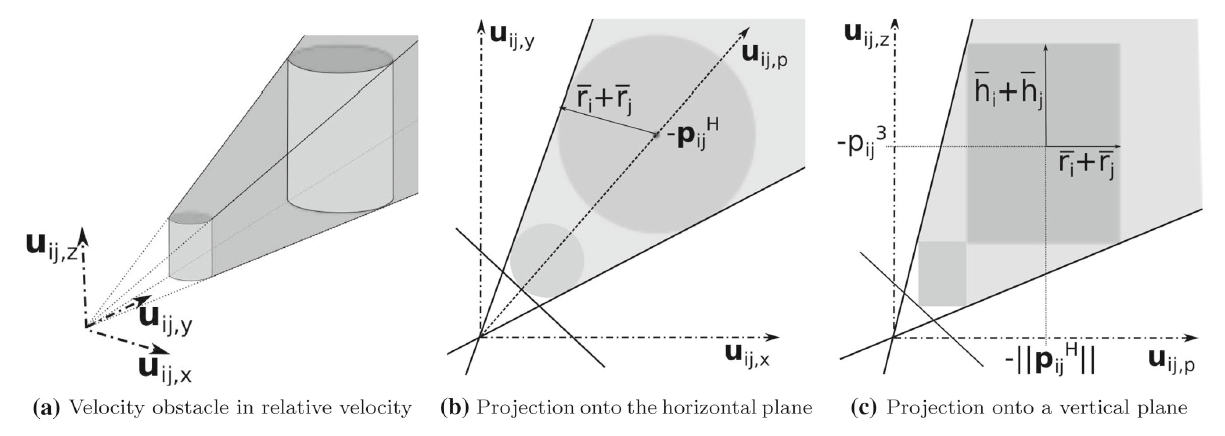
\includegraphics[width=\textwidth]{./images/velocity_obstacle.png}
\caption[Collision avoidance of a neighbouring agent using the principle of velocity obstacles]{Visualization of the interaction of two agents using velocity obstacle constraints. $\textbf{u}_i$ and $\textbf{u}_j$ are the velocities of the ego-agent and its neighbour respectively. $\textbf{u}_{ij}$ is the relative velocity. The velocities are constrained to exclude the collision region (shown in grey) \cite{alonso2015collision}}
\label{fig:vel_obs}
\end{figure}

\subsection{Nonlinear Model Predictive Control}
Collision-avoidance can be seamlessly added to nonlinear predictive control model (NMPC). Even though the high computational demand of this method, along with the complexity of the quadrotor system makes it a challenge, several fast based on Gauss-Newton methods, gradient methods, or generalized minimal residual methods has led to promising results.

Nieto et al. \cite{kamel2017robust} have successfully implemented collision-avoidance of multiple quadrotors in real time using NMPC. In this approach, the trajectory tracking and collision-avoidance is solved in a single optimization problem.This is the state-of-the-art solution for this problem and this section will be dedicated to its implementation. 

Let \textbf{x} and \textbf{u} be the state vector and control input respectively. The state transition equation:
\begin{align}
\dot{\textbf{x}}=f(\textbf{x,u})
\end{align}
The NMPC controller solves the following finite horizon optimal control problem (OCP) online at each time step.
\begin{align}
\begin{split}
\min_{\textbf{u}(t)}\quad &\int_{t=0}^{T} \left(J_x(\textbf{x}(t),\textbf{x}_{ref}(t))+J_u(\textbf{u}(t),\textbf{u}_{ref}(t))+J_c(\textbf{x}(t))\right) dt\\
s.t.\quad & \dot{\textbf{x}}=f(\textbf{x,u})\\
&\textbf{u}(t)\in \mathcal{U}\\
&\textbf{G(x}(t)) \leq 0 \\
&\textbf{x}(0)=\textbf{x}(t_0)
\end{split}
\end{align}
where, $J_x$ is the cost of deviating from the reference trajectory $x_{ref}$, $J_u$ is the penalty in control input deviation from $u_{ref}$,  \textbf{G} is the hard-constraints in the distance between agents, and $\mathcal{U}$ is the set of admissible control inputs.
\begin{align}
&J_x(\textbf{x}(t), \textbf{x}_{ref}(t)) = \Vert \textbf{x}(t)-\textbf{x}_{ref}(t)\Vert ^2\\
&J_u(\textbf{u}(t), \textbf{u}_{ref}(t)) = \Vert \textbf{u}(t)-\textbf{u}_{ref}(t)\Vert ^2
\end{align}

The collision cost $J_c(\textbf{x}(t))$ is based on a smooth collision function:
\begin{align}
J_c(\textbf{x}(t))=\sum_{j=1}^{N_{agents}}\frac{Q_c}{1+\exp\kappa_j(d_j(t)-r_{th})}
\end{align}
Where, $Q_c$ is a tuning parameter, and $r_{th}$ is a threshold distance between the agents. The parameter $\kappa_j$ decides the smoothness of the cost function. $d_j = \Vert \textbf{p}(t)-\textbf{p}(t)\Vert ^2$ is the distance to the neighbouring agent $j$. For extra safety, tight-hard constraints, $\textbf{G(x)}$, are given on the distance between two agents:
\begin{align}
\textbf{G}_j = -d_j^2+r_{min}^2
\end{align}
where, $r_{min}$ is chosen to be less than $r_{th}$ to ensure that these non-convex constraints are activated only if the the collision-potential function $J_c$ prevent the robot from approaching a hazardous situation.

In the controller, every agent predicts the future position of every other agent using a constant velocity model. To achieve this, there must be a network that communicates the current position and velocity of every agent to every other agent. The position of $j$th agent is estimated as:
\begin{align}
\textbf{p}_j(t) = \textbf{p}_j(t_0) + \textbf{v}_j(t_0)(t-t_0)
\end{align} 
Moreover, the uncertainty of the state, which is inherent to robotic applications, is propagated based on an Extended Kalman Filter (EKF).

\begin{figure}
\centering
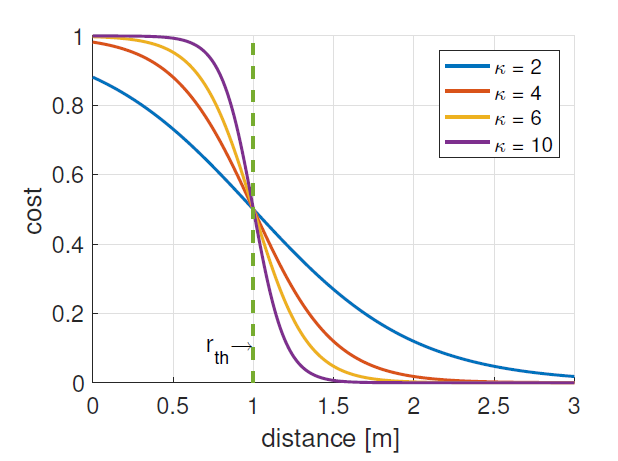
\includegraphics[width=0.6\linewidth]{./images/cost_function_nmpc}
\caption[Collision cost function vs smoothness parameter]{Variation of the collision cost function w.r.t. the smoothness parameter $\kappa$. \cite{kamel2017robust}}
\end{figure}

This method can handle priority just by modifying the \textit{connectivity graph} between agents. Agents of higher priority would not consider the collision cost with those of lower priority while performing the manoeuvre. Therefore, only lower priority agents will perform collision avoidance. Experiments and simulations showed that assigning a priority leads to smoother and faster trajectories. 


\begin{figure}
    \centering
    \begin{subfigure}[b]{\textwidth}
        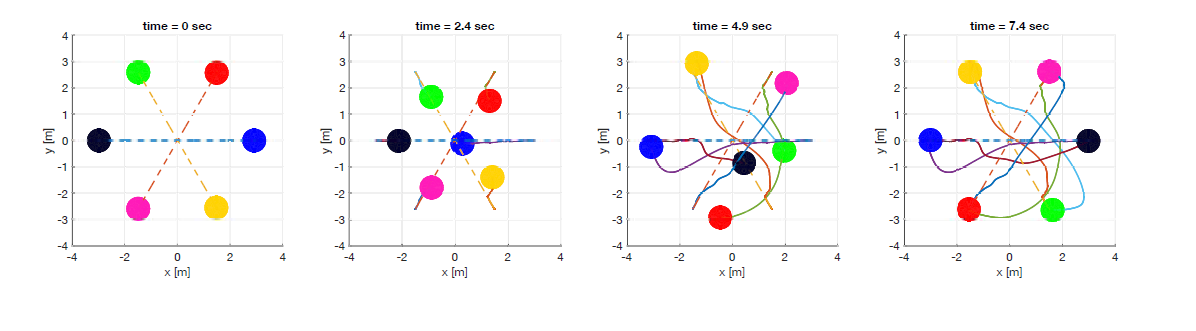
\includegraphics[width=\textwidth]{./images/collision_nmpc_1}
        \caption{No priority among agents}
        \label{fig:coll_nmpc1}
    \end{subfigure}
    \\ %add desired spacing between images, e. g. ~, \quad, \qquad, \hfill etc. 
    \begin{subfigure}[b]{\textwidth}
        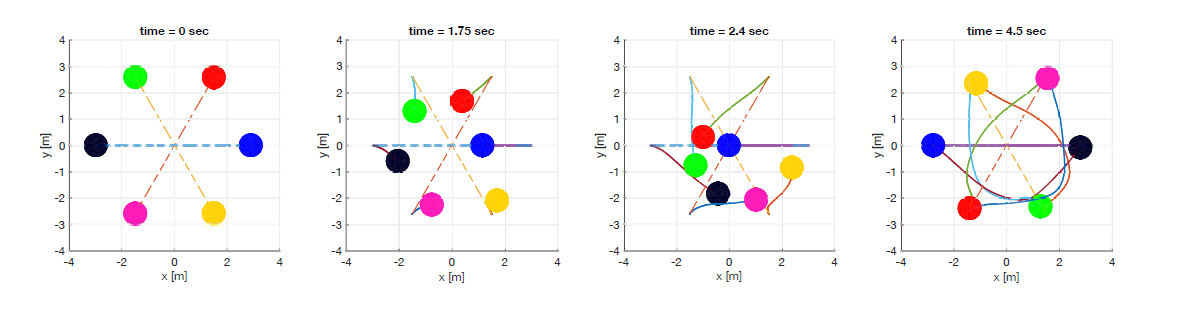
\includegraphics[width=\textwidth]{./images/collision_nmpc_2}
        \caption{Predefined priority among agents}
        \label{fig:coll_nmpc2}
    \end{subfigure}
    \caption[Position swapping of multiple agents using NMPC]{Position swapping of multiple agents using NMPC. \cite{kamel2017robust} }\label{fig:coll_nmpc}
\end{figure}

%\section{Spline-based refinement of Waypoints}
